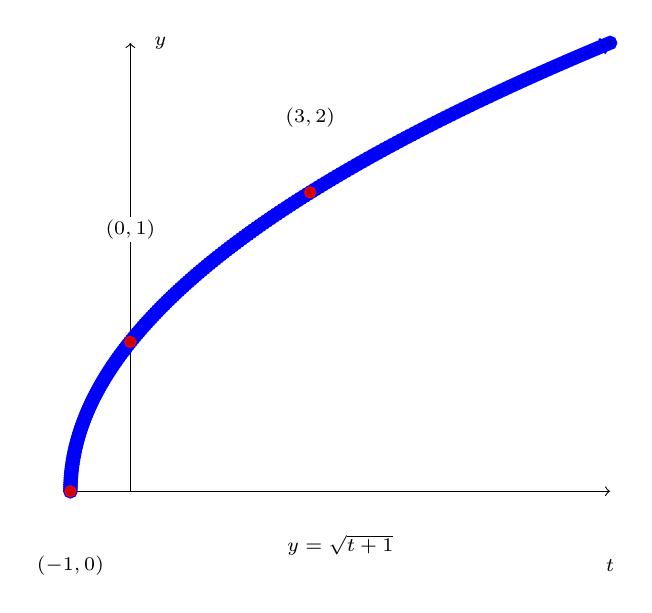
\begin{tikzpicture}
\begin{axis}[
  xmin=-1, xmax=8,
  ymin=0, ymax=3,
  axis lines=middle,
  axis line style={->},
  ticks=none,
  clip=false
]
\node at (axis cs:8,-0.5){\scriptsize $t$};
\node at (axis cs:0.5,3){\scriptsize $y$};
\node at (axis cs:-1,-0.5){\scriptsize $(-1,0)$};
% The original used gclear to clear behind the label; we emulate with a white-filled node.
\node[fill=white, inner sep=1pt] at (axis cs:0,1.75){\scriptsize $(0,1)$};
\node at (axis cs:3,2.5){\scriptsize $(3,2)$};

\addplot+[domain=0:3, samples=200, smooth, line width=1.25pt, ->, variable=\t, parametric]
  ({\t^2-1},{\t});

\addplot+[only marks, mark=*, mark size=2pt] coordinates {(-1,0) (0,1) (3,2)};

% Caption
\node at (rel axis cs:0.5,-0.12){\scriptsize $y=\sqrt{t+1}$};
\end{axis}
\end{tikzpicture}